\documentclass{article}
\usepackage{graphicx} % Required for inserting images
\usepackage{mlmodern}
\title{\huge  The Journeys of Darwin and Wallace}
\author{Sabarno Saha \\ 22MS037}
\date{April 2024}

\begin{document}

\maketitle

\section{Introduction}
\par
Charles Darwin and Alfred Russel Wallace's travels to independently establish the concept of natural selection are noteworthy milestones in the history of science. One could even argue that “Natural Selection” or “Darwinism” was the foundation on which modern biology is built. 
\section{Darwin's Journey}
\begin{figure}[h]
    \centering
    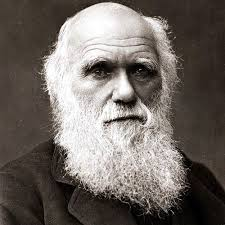
\includegraphics[width = 2.0in]{darwin.jpg}
    \caption{Charles Robert Darwin}
    \label{fig:enter-label}
\end{figure}
\par  Charles Robert Darwin, born into a wealthy English family in 1809. Something to note about Darwin was the family he was born into, Charles’ grandfather was Erasmus Darwin, the person who had written the book called Zoonomia. Zoonomia has some preliminary foundations on the common descent of species and the concept of evolution, something Erasmus’ son whould later expand, which  also gave Darwin some context and insight into the question he pondered on his voyage.The five-year expedition  on the HMS Beagle took him to various locations across the globe, including South America, the Galápagos Islands, and Australia. The Galapagos Islands were the place where Darwin was stumped by the variedness of mokingbirds in and around the islands. The voyage immediately after that gave Darwin time to reflect and formulate his theory on the origin and subsequent change of species During his travels, Darwin, being an avid naturalist and collector meticulously collected specimens, made detailed observations, and engaged in conversations with experts and locals alike. He, after experiencing an earthquake in Chile, also saw theorised that earthquakes and similar tectonic activity create and destroy landmasses. Thus he and later wallace could explain why biogeography was important to their theory.  \\ 
\begin{figure}[h]
    \centering
    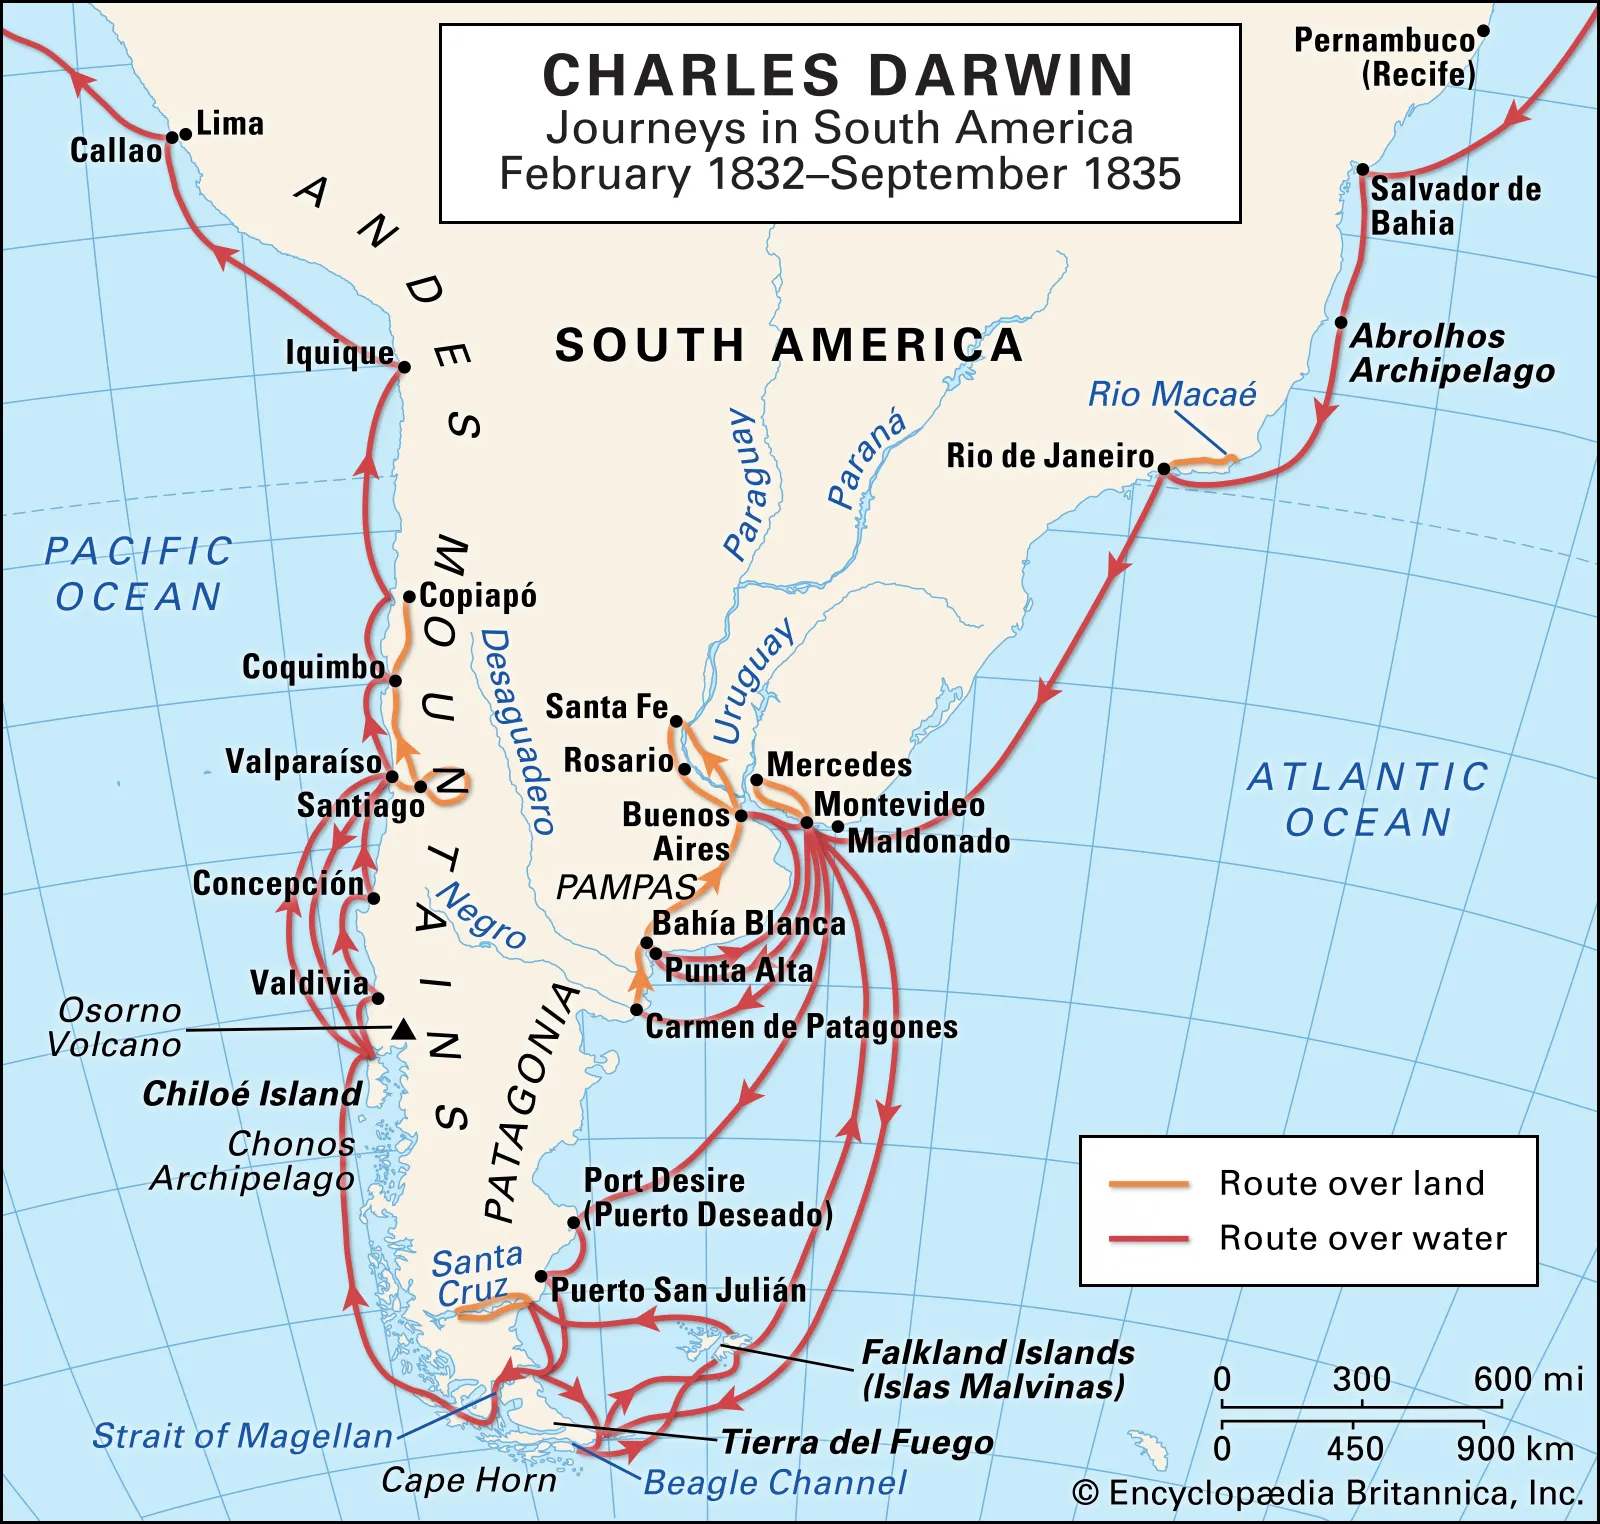
\includegraphics[width = 3.0in]{map-journeys-Charles-Darwin-South-American-September-1835.jpg}
    \caption{Darwin's Journey of the HMS Beagle}
\end{figure}
\par 
Darwin’s journey was an important one as he formulated the theory using the mockingbirds and fossils sloths he found in the shores of south America. The giant fossils he discovered of the common ancestor to the armadillo was hinting at the fact that species could infact change. The pre-existing theory of special creation was slowly being disregarded by Darwin. He was slowly starting to see that species could change, which gave birth to a fear in him. The fear of being disregarded by the scientists and the church back then, which was the reason he chose to keep the discovery a secret for such a long time, until Wallace forced his hand to show everyone his and Wallace’s discovery. After a long time in which Darwin kept hsi theory secret only between him and his friends, he and Wallace jointly presented their findings together on the same day in a reading in front of the Royal Society. He then published his own book titled, “ The Origin of Species” which became a hit with the people back then and was accepted by them over the prevalent theory of special creation.

\section{Wallace's Journey}
\begin{figure}[h]
    \centering
    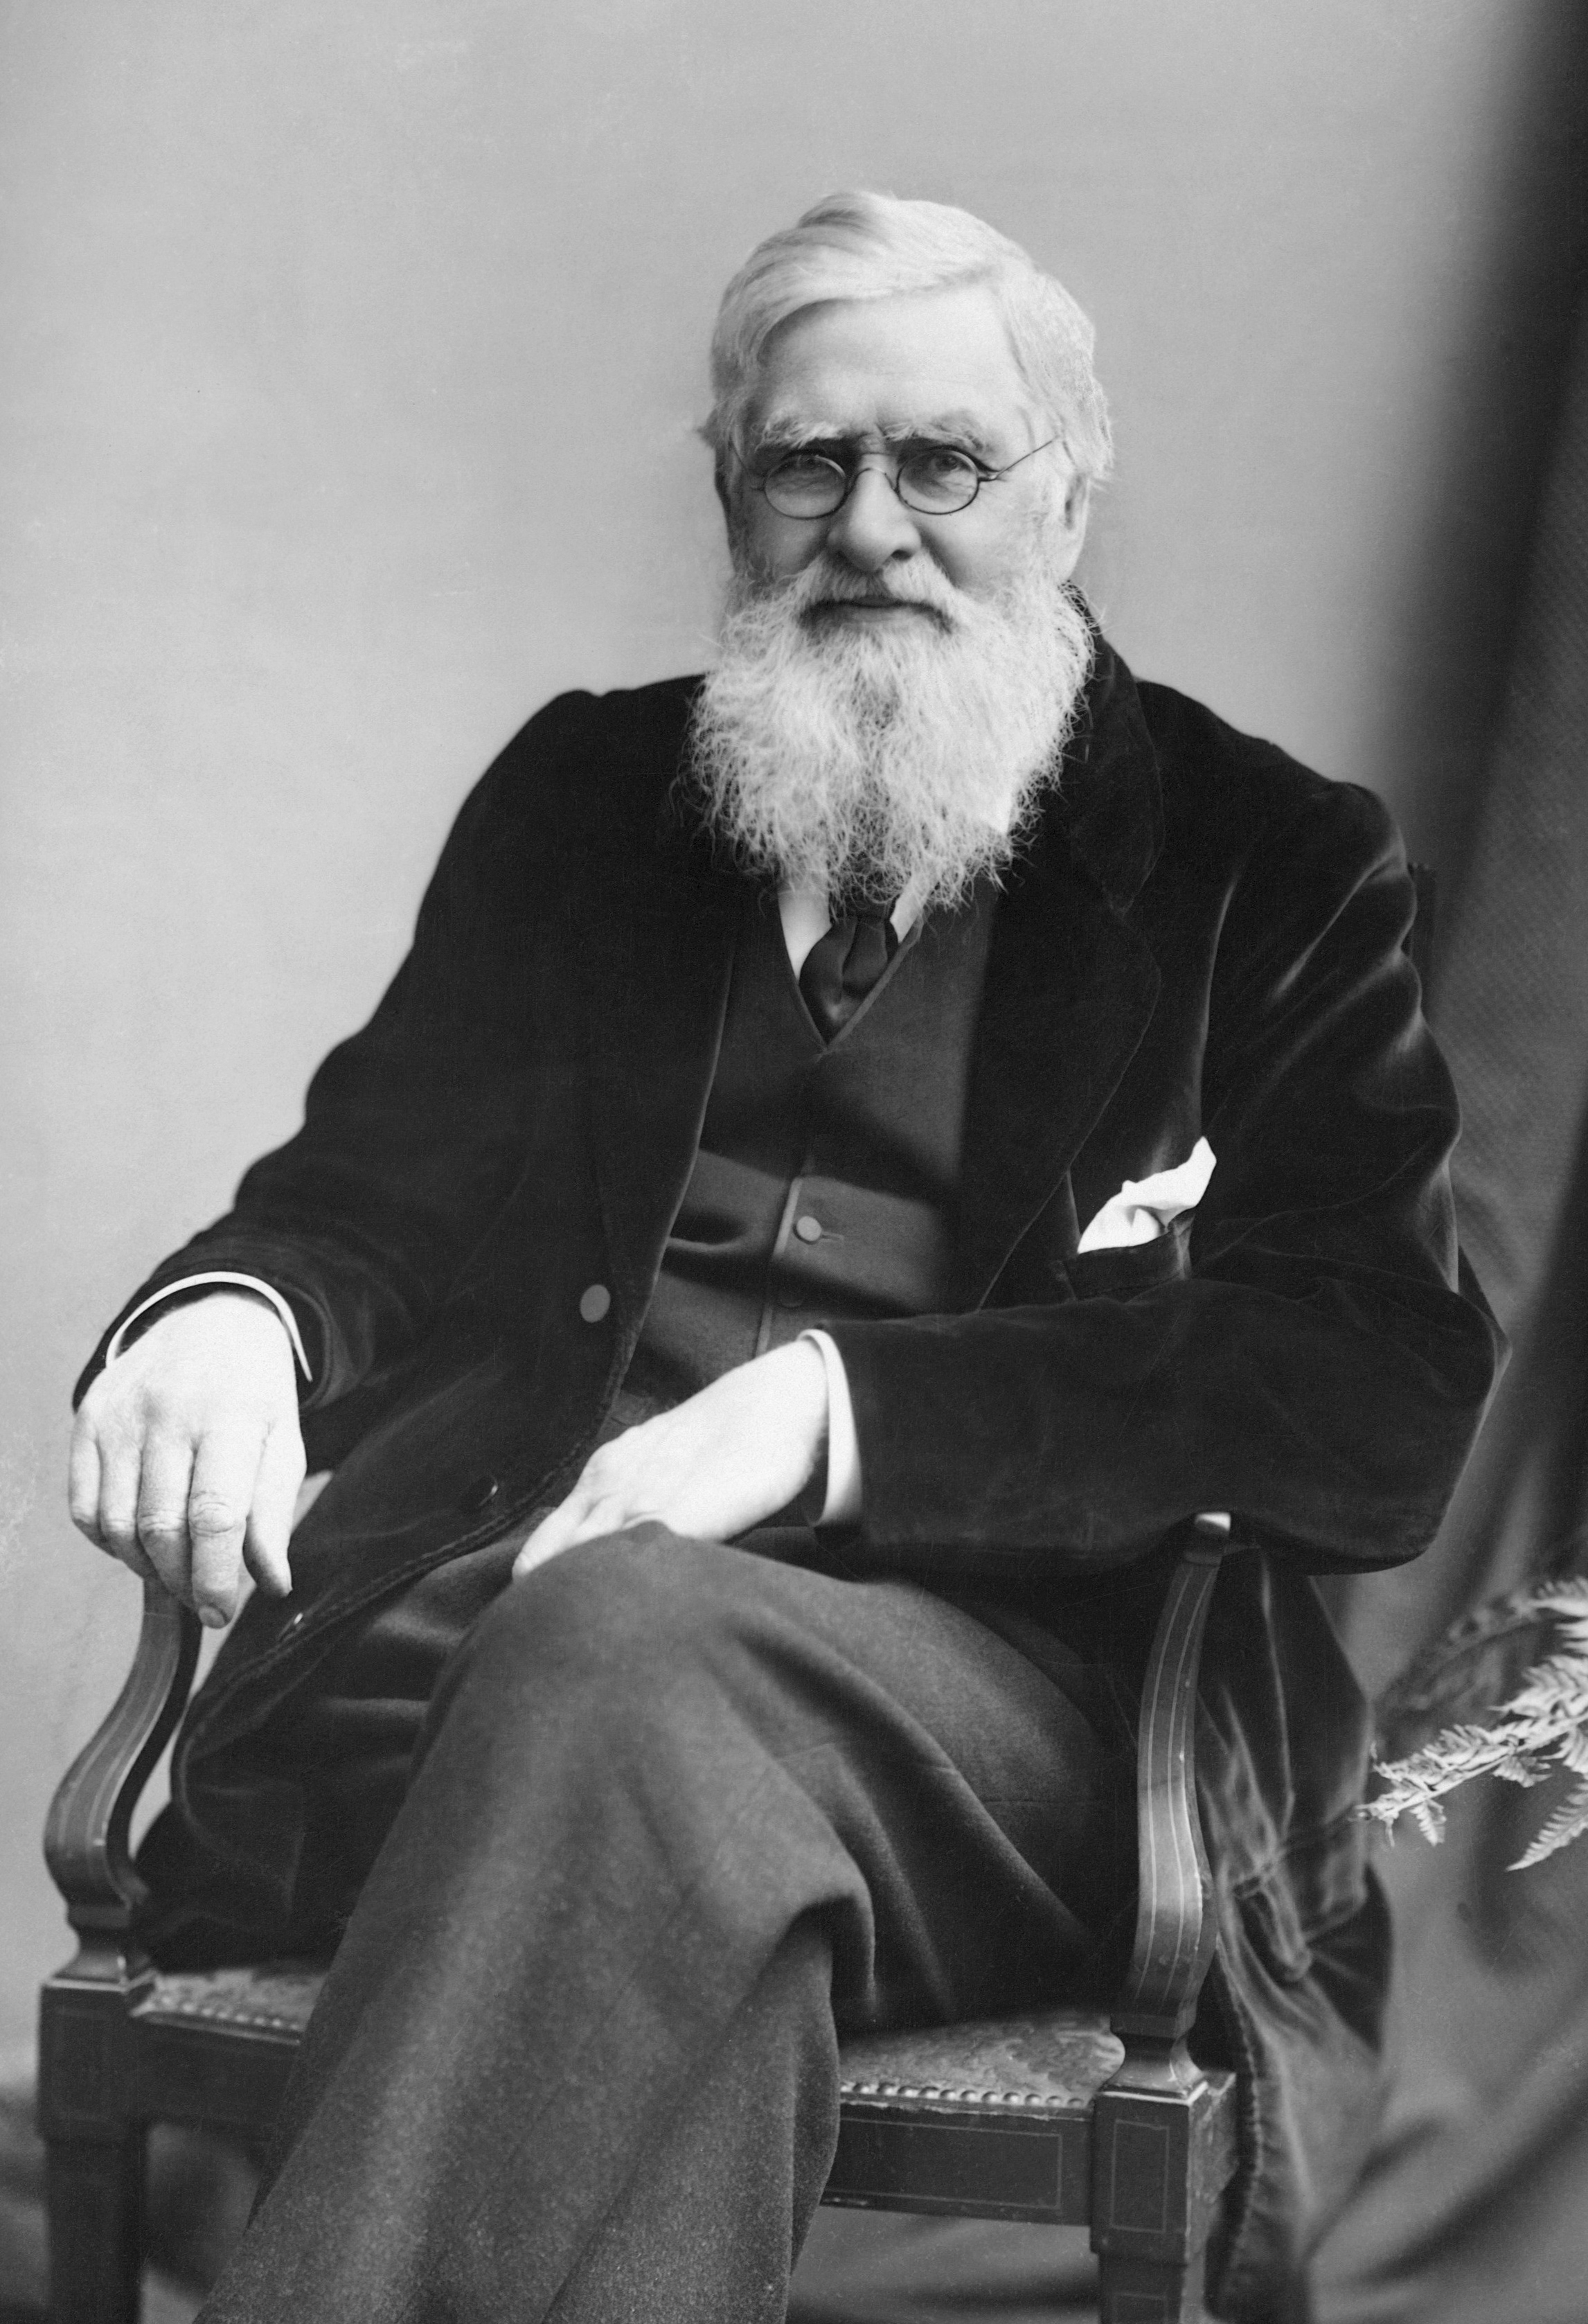
\includegraphics[width = 3.0in]{Alfred-Russel-Wallace-c1895.jpg}
    \caption{Alfred Russell Wallace}
\end{figure}
\par 
Alfred Russel Wallace, a contemporary of Darwin, was born in 1823 in Wales to a radically different socio-economic family. His parents were middle class and not high upper class like Darwin’s. He joined an apprenticeship under his brother later as land surveyor, a skill which undoubtedly helped him later. He read voraciously at the London Mechanics Institute and became a collector of natural specimens there. This interest in collection of natural species, mostly butterflies led him to travel and independently formulate the theory that would later be called Darwinism in his own words. Soon, he would also embark on a Voyage to the Malay Archipelago to discover the variety of mammals and marsupials living on either side of the fictituous line, now dubbed the Wallace line. \\ 
\begin{figure}[h]
    \centering
    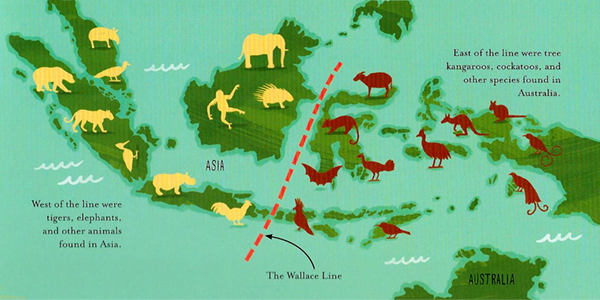
\includegraphics[width =5.0in]{wallaceline.jpg}
    \caption{Wallace Line}
\end{figure}

During his time in the Malay Archipelago, Wallace made numerous significant discoveries, including the concept of biogeography and the Wallace Line, a fictitious boundary separating the fauna of Asia and Australia. His own discoveries came observing the fact that on certain islands which were on the left side  had more mammals, while those on the right on the right side had more marsupials. Now the left islands shared more fauna with the Asia, and the right shared more with Australia. It was later known that the left islands were at some point connected to Asia and the right to Australia. Thus the Wallace line was born. Now he could see that animals from different continents hopped onto those islands and later changed slightly within the same species. His fever dream ultimately resulted in him penning down his ideas and sending a letter to Darwin, who saw it and then decided to publish his own findings as well together with Wallace in the Royal Society of London.

\section{Conclusion}
In conclusion, the journeys of Charles Darwin and Alfred Russel Wallace to their discoveries of natural selection represent extraordinary feats of exploration, observation, and perseverance in collecting a large number of samples and then observing very subtle and minute differences. This is how the great minds formulated possibly the greatest theory in modern biology has seen or will ever see.

\end{document}
